\section{測定結果}

\subsection{信号の大きさ}
測定した結果からx軸が印加電圧、y軸が信号の大きさのグラフを作成した。
図\ref{fg:PIN_MPVvsBias} は増幅層の無いPINの信号の大きさの電圧依存性で、図\ref{fg:APD_MPVvsBias} はLGAD検出器の信号の大きさの電圧依存性である。
PINの信号の大きさの電圧依存性を見ると、電圧をかけ始めた領域では、電圧を上げると信号の大きさが上昇していることがわかる。
さらに電圧を上げていくと、信号の上昇率が徐々に減少し、信号の大きさが約25mVでほぼ一定になった。
これは、電圧をかけ始めた領域では、バルクの空乏層が電圧を上げることで拡大するため、信号の大きさが上昇していると考える。
また、信号の大きさが約25mVでほぼ一定になった理由は、バルクが全て空乏化したことにより、
これ以上電圧を大きくしても空乏層は拡大しないためであると考える。
LGAD検出器の信号の大きさの電圧依存性を見ると、電圧を上げると信号の大きさが指数関数的に増大していることがわかった。
この結果より、増幅層の高電場によって、荷電粒子が入射することで生成された電子正孔対が増幅されることがわかった。

\begin{figure}[h]
    \begin{minipage}[b]{0.5\linewidth}
        \centering
        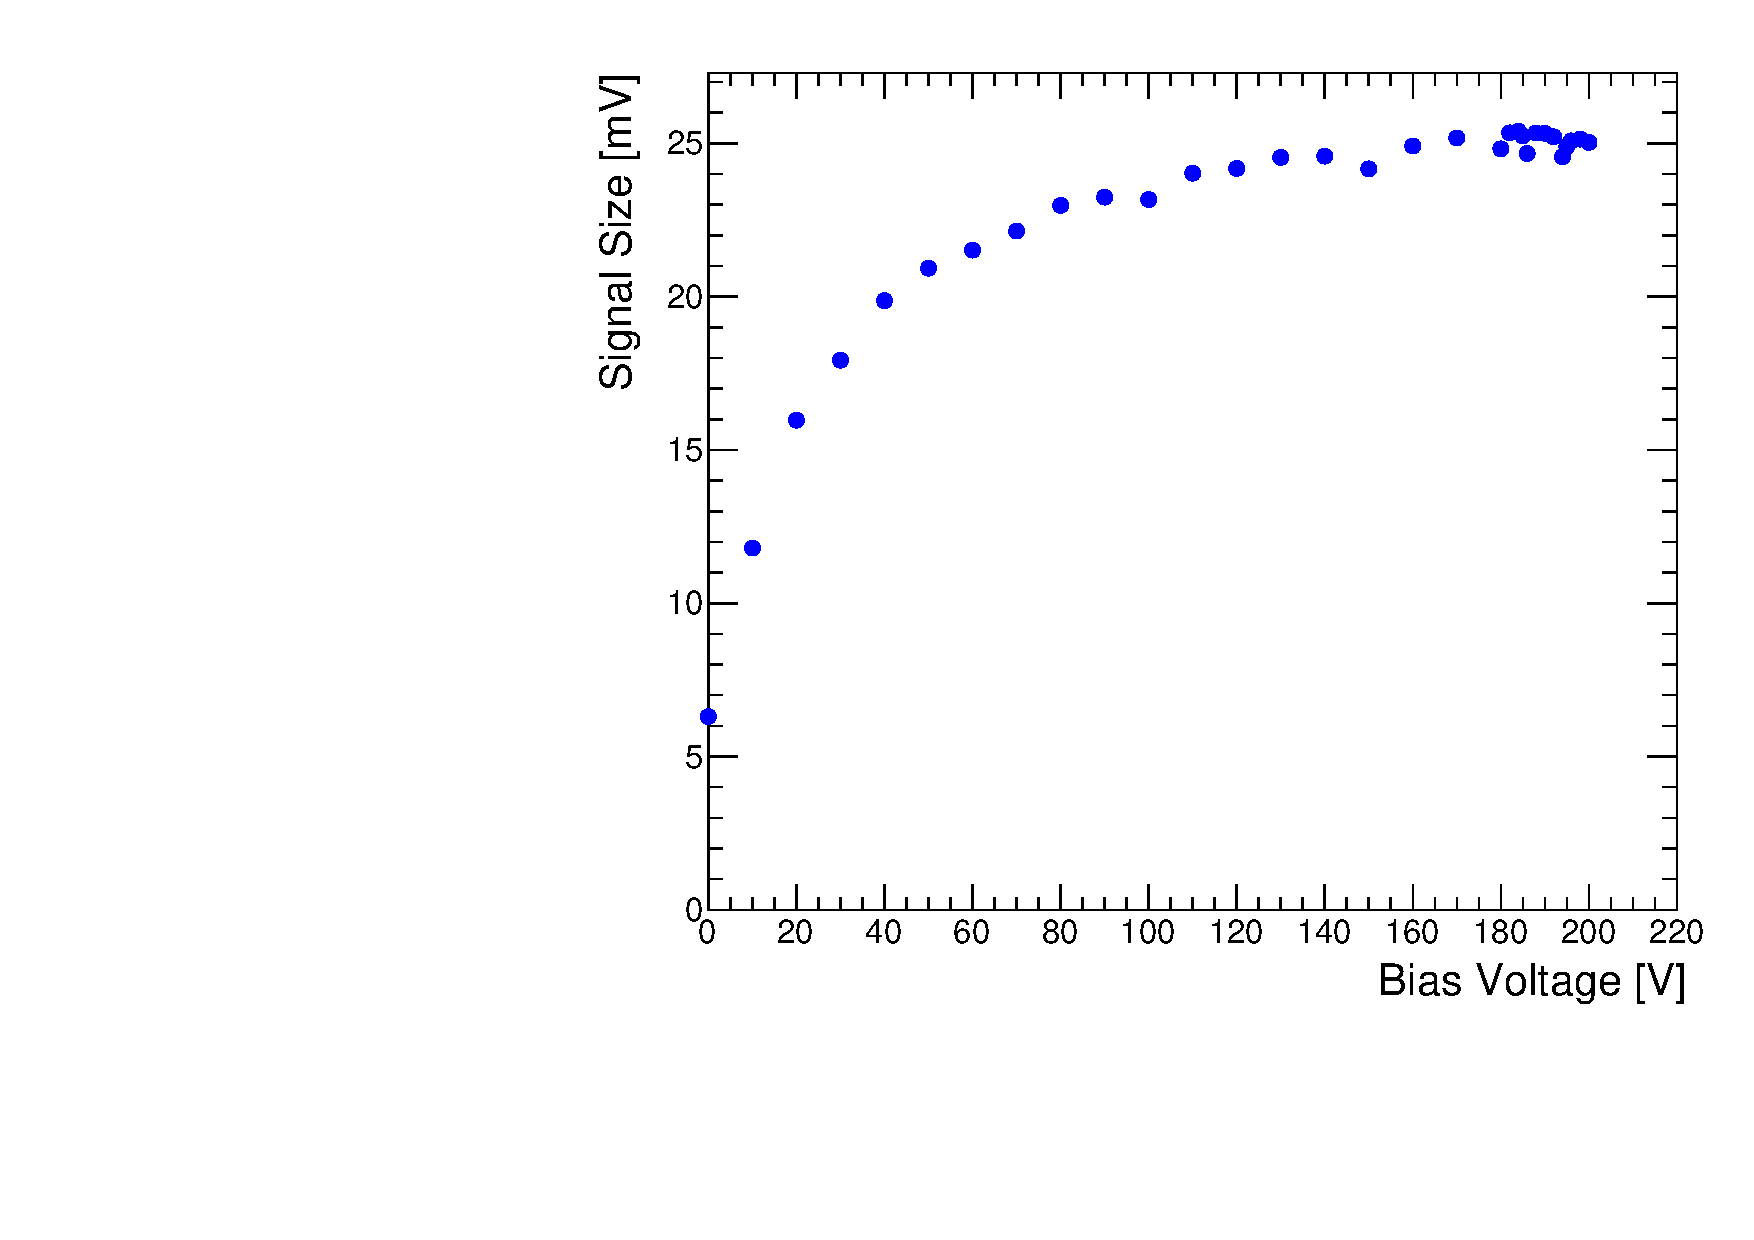
\includegraphics[width=8cm]{fig/graph/PhvsVoltage_PIN.pdf}
        \subcaption{増幅層が無いPIN}
        \label{fg:PIN_MPVvsBias}
    \end{minipage}
    \begin{minipage}[b]{0.5\linewidth}
        \centering
        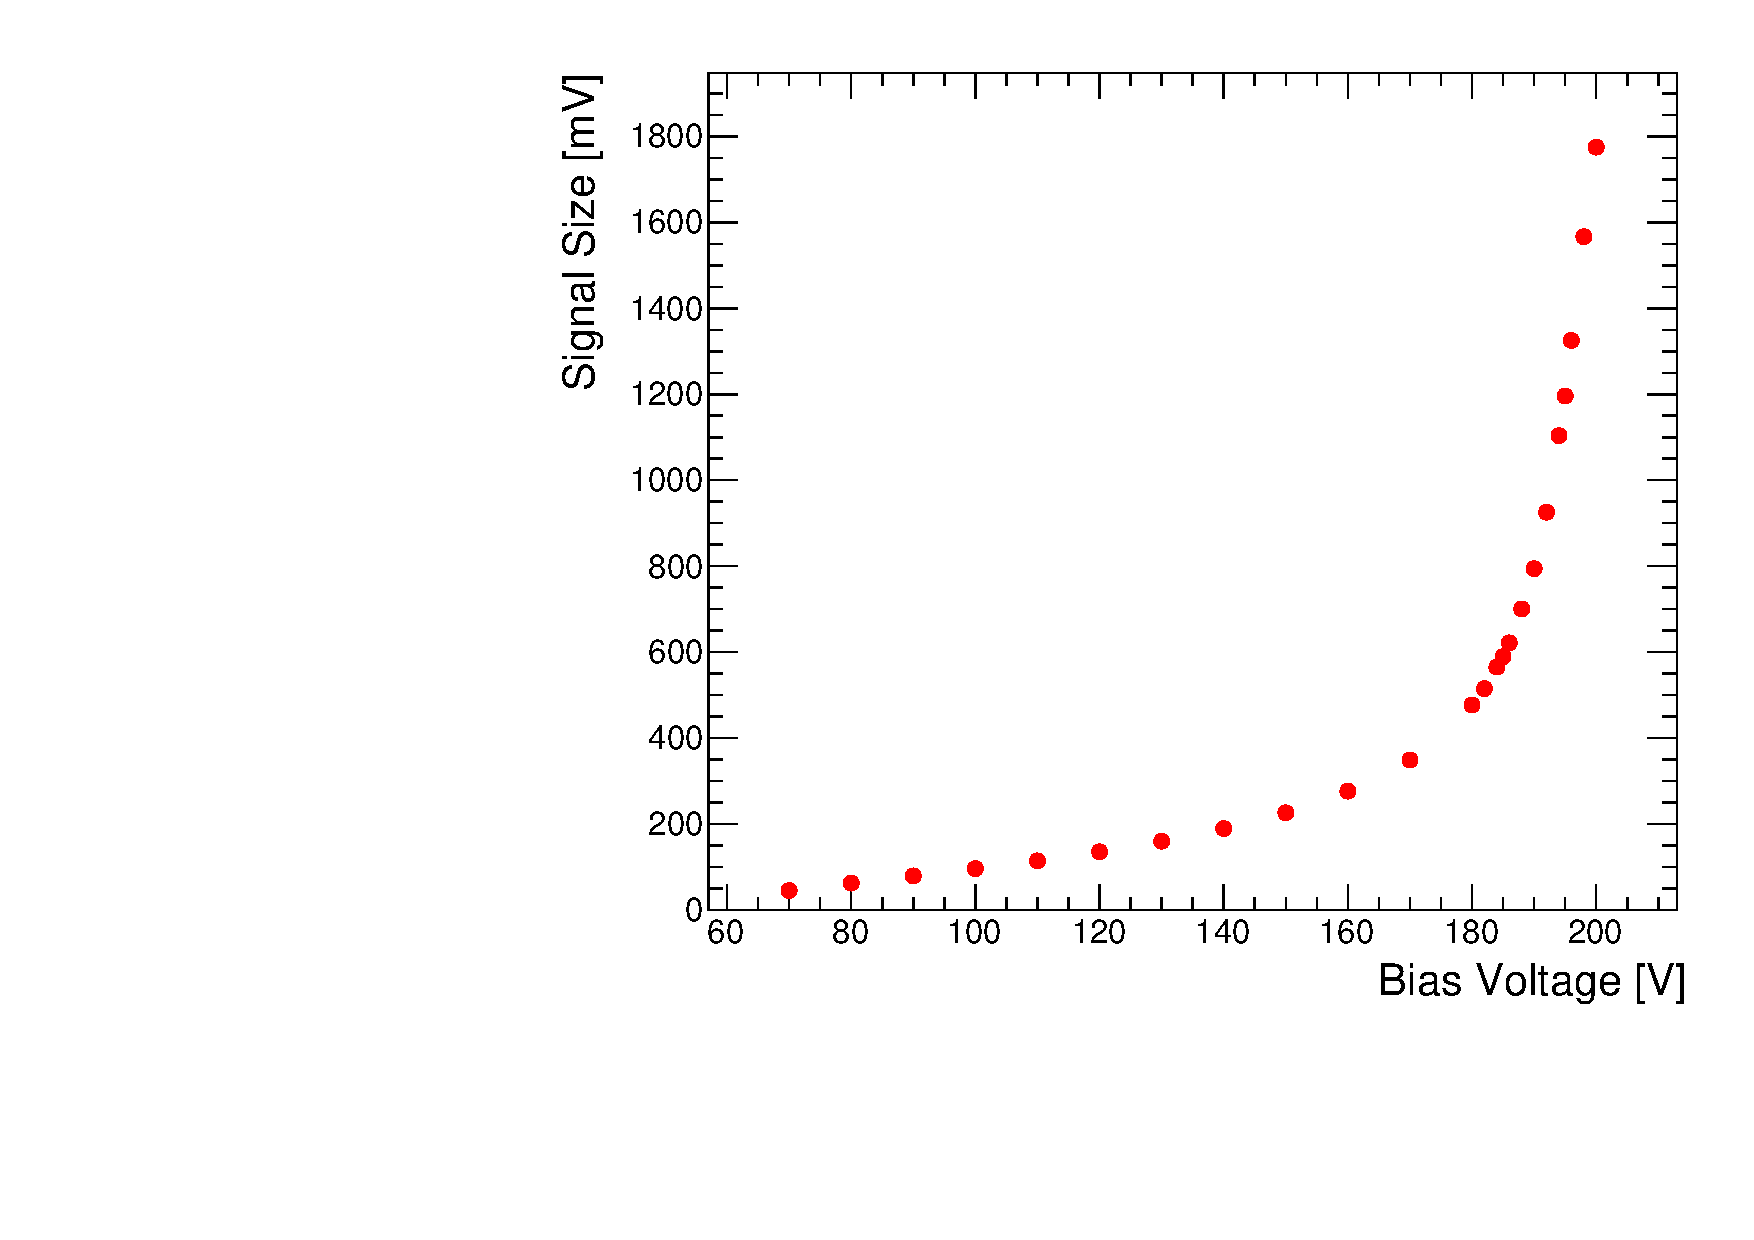
\includegraphics[width=8cm]{fig/graph/PhvsVoltage_APD.pdf}
        \subcaption{増幅層が有るLGAD検出器}
        \label{fg:APD_MPVvsBias}
    \end{minipage}
    \caption[AC-LGAD検出器の信号の大きさの電圧依存性]{AC-LGAD検出器の信号の大きさの電圧依存性\\x軸が電圧でy軸が信号の大きさ}
\end{figure}

\subsection{時間分解能}
時間分解能$\sigma_t$の電圧依存性を以下の 図\ref{fg:TresovsBias} に示す。
青点がPINと赤点がLGAD検出器の測定結果を、同時にx軸が電圧、y軸が時間分解能のグラフにプロットした様子になっている。
PINの時間分解能は、電圧を印加し始めたところでは向上していることがわかった。
PINは電圧を上げることで空乏化により空乏層が拡大し、信号が大きくなるため、時間分解能が向上したと考える。
また、時間分解能の向上割合が小さくなるのは、印加電圧の上昇による空乏層の拡大がほとんど起こらなくなったためであると考える。
LGAD検出器の時間分解能は188〜192 Vでおよそ10 psを得られることがわかった。この電圧を超えると時間分解能が悪化する様子を見ることができた。
そのため、188〜192 Vが本実験の測定セットアップでのセンサーの運転電圧であると考える。
%時間分解能の最小値の統計誤差の範囲内に、時間分解能がある時の電圧を、本実験の測定系におけるAC-LGAD検出器の運転電圧とすると、188 Vと190 Vがその範囲内にあることがわかった。
%180 Vから200 Vの範囲は2 Vずつ測定を行なっていたので、運転電圧は1 Vの誤差があると考えると、運転電圧は $189 \pm 2$ Vであった。
運転電圧を超える電圧を印加すると、時間分解能が悪化してしまう原因については第4章で詳しく調べる。
LGAD検出器とPINの時間分解能の比較から、検出器に増幅効果があることで時間分解能が5倍程度に改善することがわかった。

\begin{figure}[h]
    \centering
    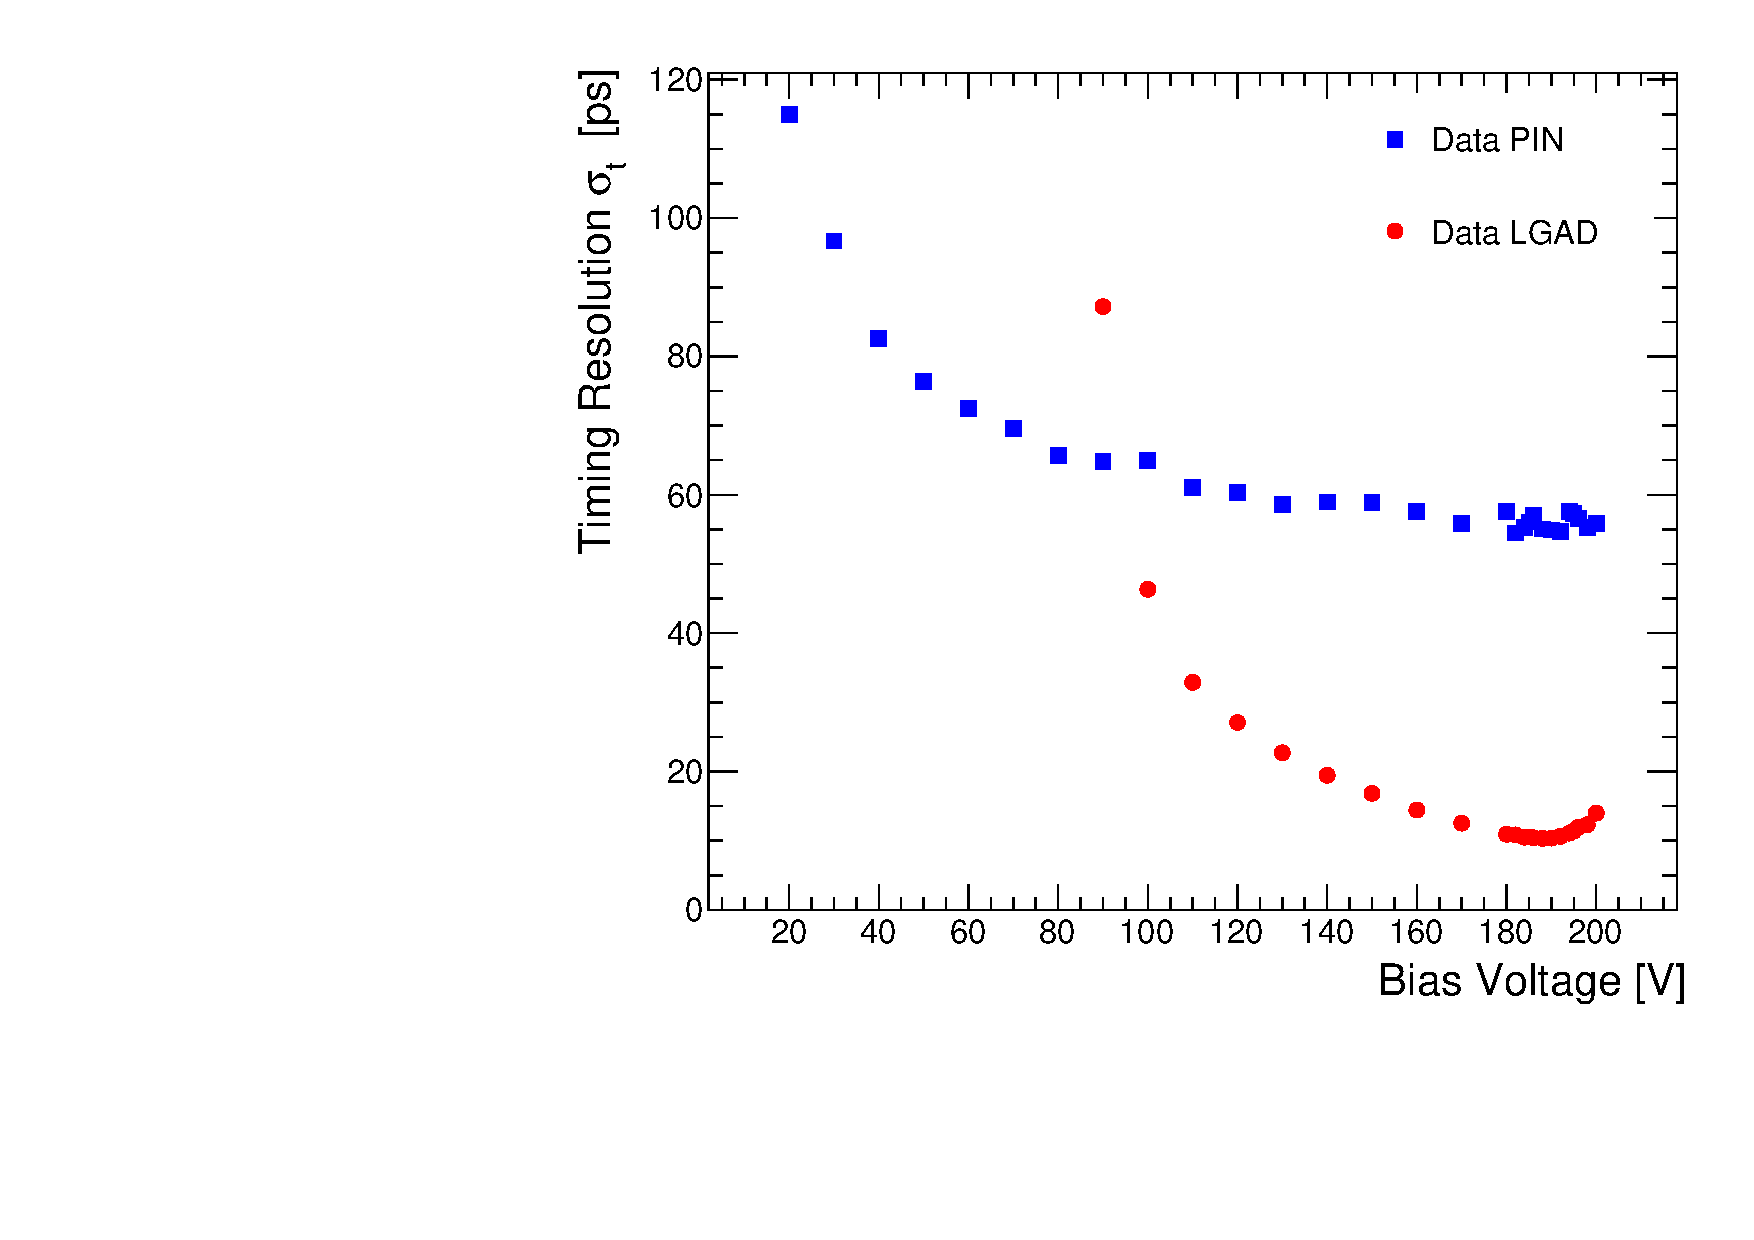
\includegraphics[width=8cm]{fig/graph/TresovsVoltage.pdf}
    \caption[AC-LGAD検出器の時間分解能$\sigma_t$の電圧依存性]{AC-LGAD検出器の時間分解能$\sigma_t$の電圧依存性\\x軸が電圧でy軸が時間分解能、青点がPINで赤点がLGAD}
    \label{fg:TresovsBias}
\end{figure}

\subsection{増幅率}
LGAD検出器とPINの信号の大きさから、AC-LGAD検出器の信号の増幅率を求めた。図\ref{fg:Gain_TresovsBias} は、
求めた増幅率とLGADの時間分解能の測定結果の電圧依存性を同時にプロットしたものになっている。
%x軸が電圧で、y軸が増幅率と時間分解能を示している。赤点が時間分解能で、青点が増幅率、黒線が増幅率のフィット結果である。
この図を見ると、増幅率は電圧を上げることで増大することがわかった。
これは、印加電圧を増やしたことによるPINの信号の大きさの増加と比べて、LGADの信号の大きさの増加が非常に大きいためである。
運転電圧188〜192Vの範囲の増幅率求めた。
以上の結果より、AC-LGAD検出器の時間分解能が最も良い増幅率は、 およそ20〜35 倍であることがわかった。

\begin{figure}[H]
    \centering
    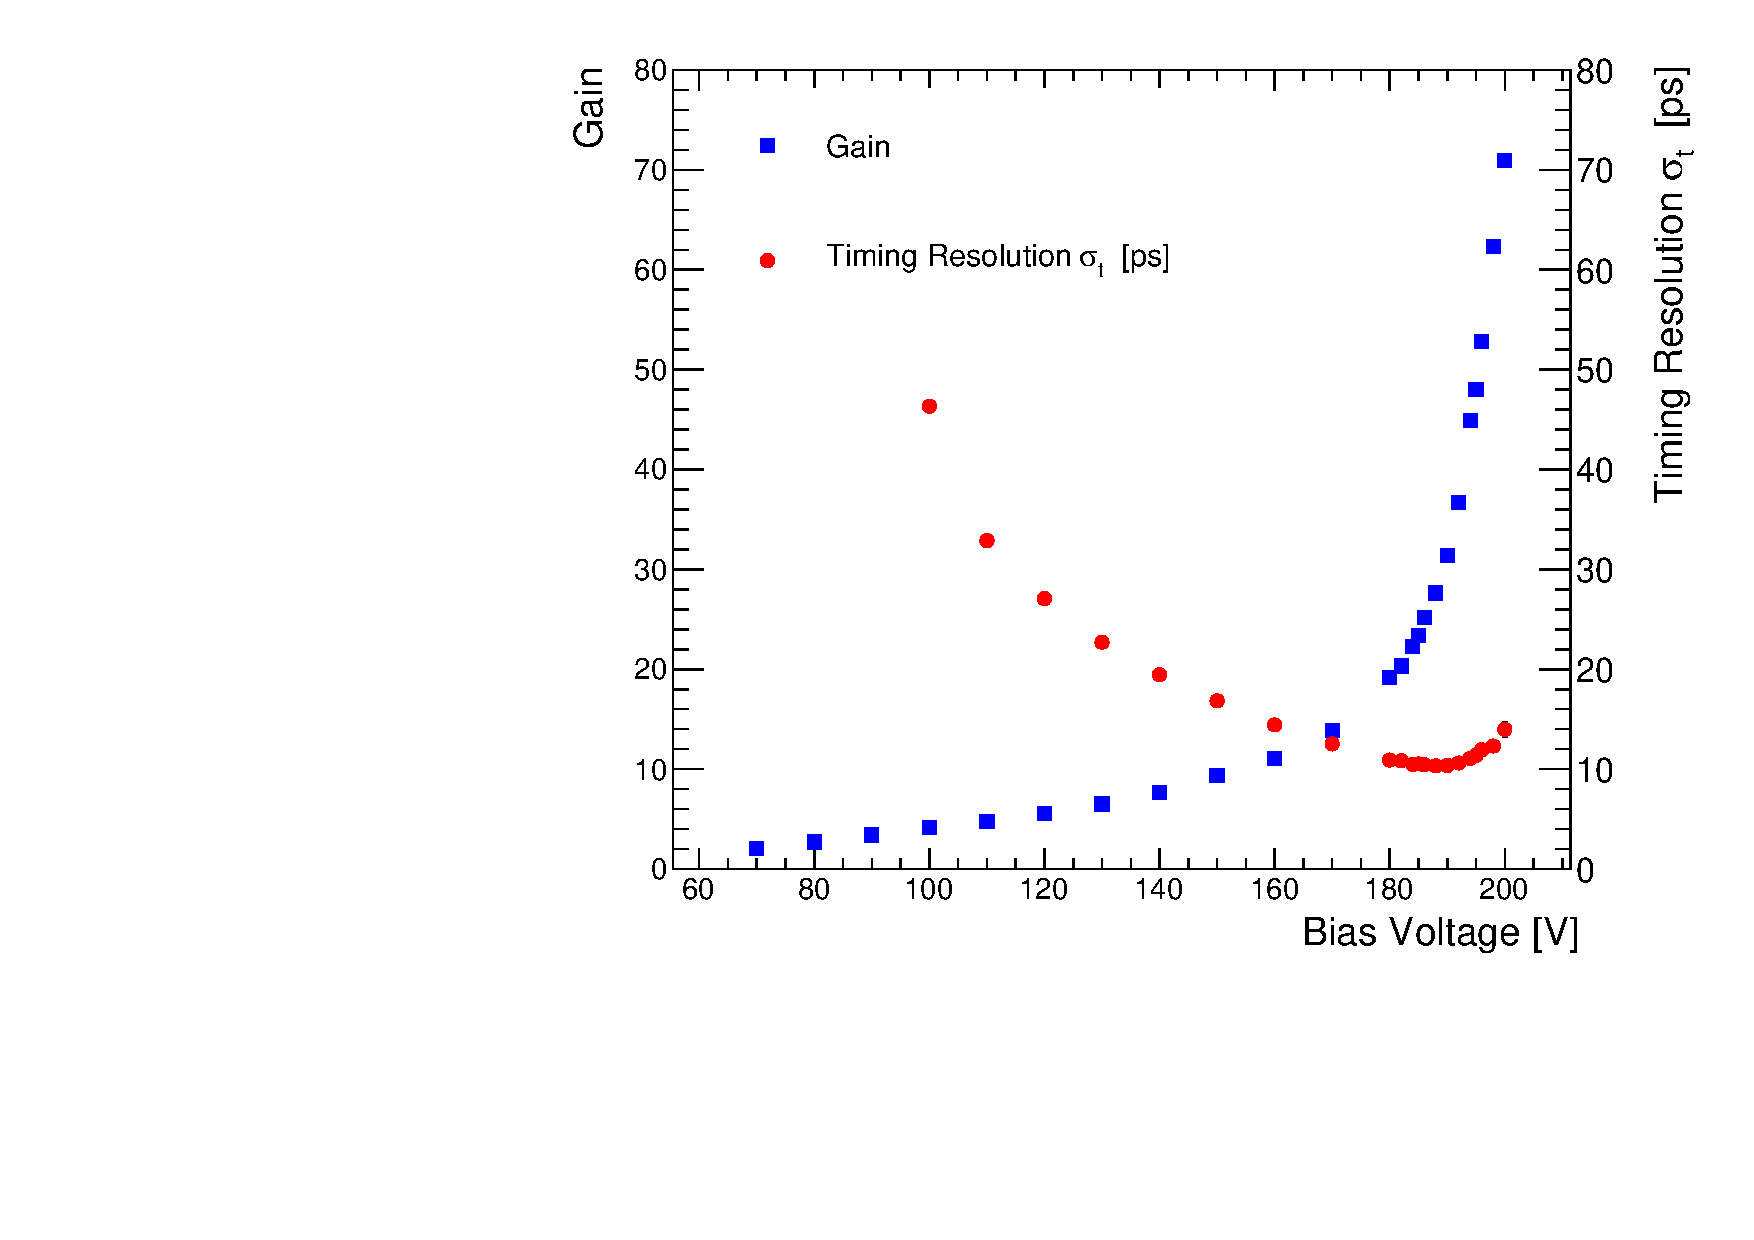
\includegraphics[width=10cm]{fig/graph/Gain_TresovsVoltage_APD.pdf}
    \caption[AC-LGAD検出器の増幅率と時間分解能の電圧依存性]{AC-LGAD検出器の増幅率と時間分解能の電圧依存性\\x軸が電圧でy軸が増幅率と時間分解能、赤点が増幅率、青点が時間分解能}
    \label{fg:Gain_TresovsBias}
\end{figure}
